\documentclass{article}
\usepackage{amsmath,amssymb}
\usepackage{color}
\usepackage{graphicx}
\usepackage{geometry}
\linespread{1.6}
\geometry{a4paper,left=2cm,right=2cm,top=1cm,bottom=1cm}

\begin{document}

\section{Geomatric explaination of matrix}

\subsection{Two geometric ways understanding matrix}

For linear equations:
\begin{equation}
\label{eq:3}
\begin{cases}
2x - y = 0 \\
-x + 2y = 3
\end{cases}
\end{equation}

We can write them in matrix multiplication form:
\begin{equation}
\label{eq:2}
\left[ \begin{array}{cc}
2 & -1\\
-1 & 2
\end{array} \right]
\left[ \begin{array}{c}
x\\y
\end{array} \right] = \left[ \begin{array}{c}
0\\3
\end{array} \right]
\end{equation}
where  $\boldsymbol{A}$ is the coefficient matrix, $\boldsymbol{x}$ is the
unknown variable vector, $\boldsymbol{b}$ is the result vector, written as $\boldsymbol{Ax=b}$.

Such kind of form can be understood from two geometric ways:

(1) Row picture form:
It plots every row function. In two dimentional example they are two linear
equations, each with two unknown variables, i.e. two lines.

(2) Column picture form:
The plot is presented in column vector way. The purpose is to find a linear
combination that gives the column $\boldsymbol{b}$. Applying all possible
combinations of \textit{x} and \textit{y} produces the two dimentional plane.
But in this case there is only a unique set combination produces $\boldsymbol{b}$.

\begin{figure}[h]
  \centering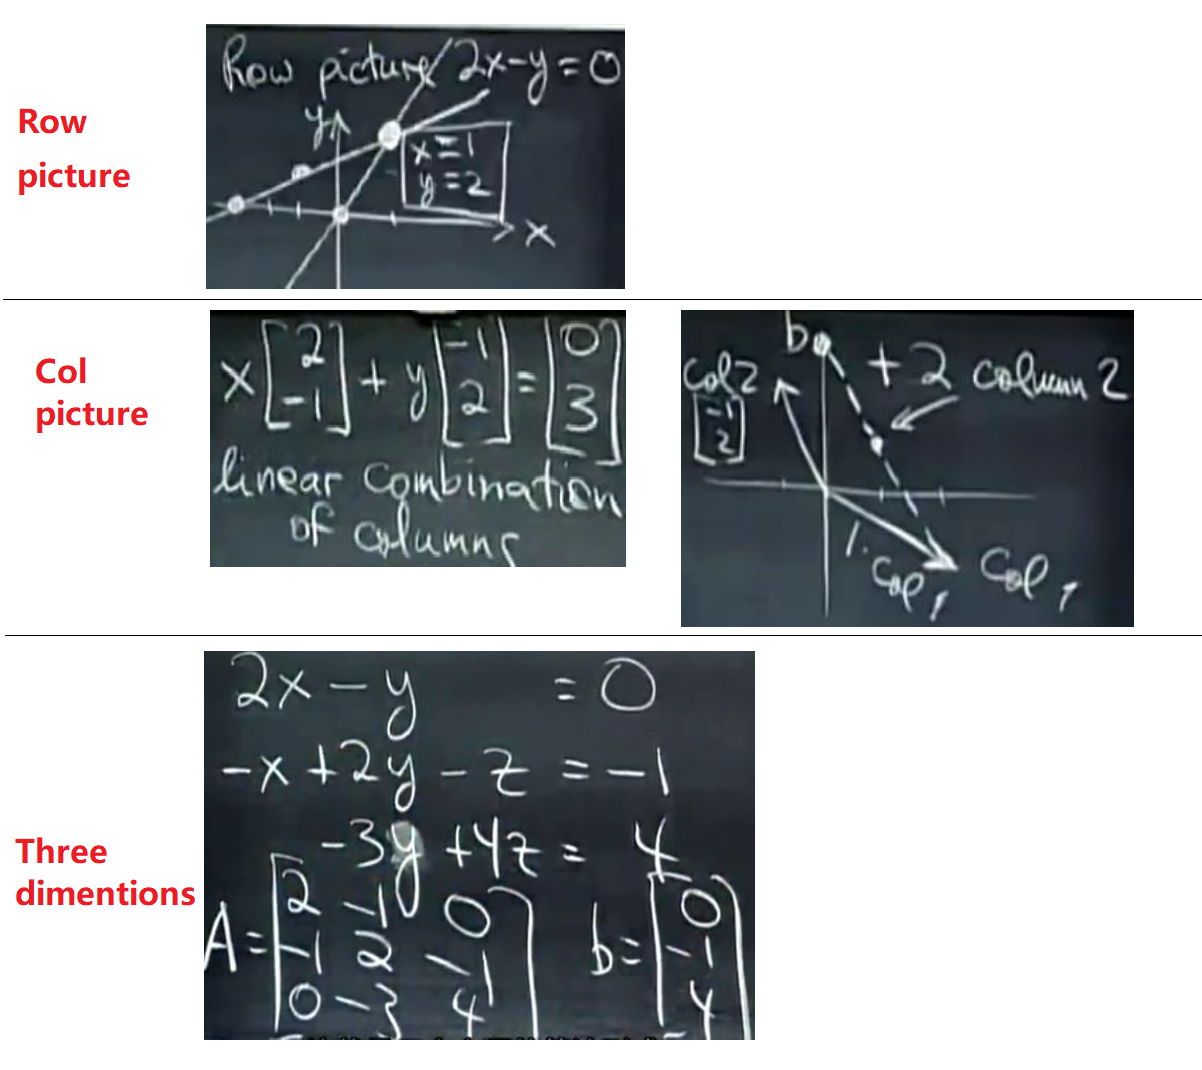
\includegraphics[scale=0.45]{figures/1.png}
\end{figure}

The above interpretation applies to higher dimentional examples.

\subsection{The roots of equation sets}
Taking the above three dimentional equation sets as example: when
$\boldsymbol{b}$ is unknown (and the $\boldsymbol{Ax}$ remain unchanged),
whether there is solution for every $\boldsymbol{b}$?

From the column picture explaination, this question is an equavlent of: whether
the linear combinations of columns in $\boldsymbol{A}$ fill up a three
dimentional space?

Answer:
The above case is non-singular matrix, so YES.
For general case, the equation sets {\color{red} only has solution when $\boldsymbol{b}$ is
in the column space spaned by $\boldsymbol{A}$ }.

There are many benefits to consider matrix multiplication in {\color{red} column
  picture} way.

\subsection{Appendix}


\end{document}
